%\documentclass[11pt,a4paper]{article}
\documentclass{article}
\usepackage{arxiv}

%%%%%%% META STUFF %%%%%%%%%%%%%%%
\usepackage{xifthen}
\usepackage{xparse}
\usepackage{lipsum}
%%%%%%%%FONT%%%%%%%%%%%%%%%%%%%%%%
\usepackage[utf8]{inputenc}
\usepackage[T1]{fontenc}    % use 8-bit T1 fonts
\usepackage{microtype}
\usepackage{upgreek}
%\usepackage{lmodern}
%\usepackage[english]{babel}

%%%%%%%LAYOUT%%%%%%%%%%%%%%%%%%%%%%%%
%\usepackage{a4wide}
\usepackage[hang]{footmisc}

%\usepackage[nofoot, left=2.20cm, bottom=1.5cm, right=2.20cm, top=2.5cm]{geometry}
%\usepackage{parskip} % automatic line breaks
\usepackage{enumitem}
\usepackage{subcaption}
\usepackage{tabularx}
\usepackage{longtable}
\usepackage{floatrow}
\usepackage{array}
\newcolumntype{|}{!{\vrule width 0.5pt}}
\newfloatcommand{capbtabbox}{table}[][\FBwidth]
\usepackage{booktabs}

%%%%%GRAPHICS%%%%%%%%%%%%%%%%%%%%%%%%%%%
\usepackage{float} % https://ctan.org/pkg/float
\usepackage{graphicx}  % For including images
\graphicspath{{../code/figures/}}
% do not move figures across sections
\usepackage[section]{placeins}

%%%%%%%%% color %%%%%%%%%%%%%%%%%
\usepackage{xcolor}
\definecolor{mygray}{HTML}{F7F7F7}

%%%%%%%%%%||bibliography||%%%%%%%%%%%%%
\usepackage{natbib}
\usepackage[nottoc,numbib]{tocbibind}
\usepackage{doi}
\nocite{*}
%\usepackage[maxbibnames=4,backend=biber,style=alphabetic, autocite=footnote]{biblatex}
%\usepackage{apacite} % https://ctan.org/pkg/apacite
%\setlength\bibitemsep{0.4\baselineskip}
%\DeclareFieldFormat{url}{URL\addcolon\space\url{#1}}
%\DeclareFieldFormat{isbn}{ISBN\addcolon\space{#1}}
%\DeclareFieldFormat{doi}{%
%    DOI\addcolon\space
%    \ifhyperref
%    {\href{https://doi.org/#1}{\nolinkurl{#1}}}
%    {\nolinkurl{#1}}%
%}

%%%%%%MATH%%%%%%%%%%%%%%%%%%%%%%%%%%%
%\usepackage{amsfonts}
%\usepackage{amsmath}
\usepackage{mathtools}
\usepackage{amssymb}
\usepackage{latexsym}
\usepackage{dsfont}
\usepackage{nicefrac}       % compact symbols for 1/2, etc.
\usepackage{bm}
\usepackage{siunitx}

%\usepackage{mathpazo}
%\allowdisplaybreaks

\newcommand{\abs}[1]{\lvert #1 \rvert}
\newcommand{\norm}[1]{\left\lVert#1\right\rVert}
\DeclareMathOperator*{\argmax}{arg\,max}
\DeclareMathOperator*{\argmin}{arg\,min}
% Left-right bracket
\newcommand{\lr}[1]{\left (#1\right)}
% Left-right square bracket
\newcommand{\lrs}[1]{\left [#1 \right]}
% Left-right curly bracket
\newcommand{\lrc}[1]{\left \{#1\right\}}
% Left-right absolute value
\newcommand{\lra}[1]{\left |#1\right|}
% Left-right upper value
\newcommand{\lru}[1]{\left \lceil#1\right\rceil}
% Scalar product
\newcommand{\vp}[2]{\left \langle #1 , #2 \right \rangle}
% The real numbers
\newcommand{\R}{\mathbb R}
% The natural numbers
\newcommand{\N}{\mathbb N}
% Expectation symbol with an optional argument
\NewDocumentCommand{\E}{o}{\mathbb E\IfValueT{#1}{\lrs{#1}}}
% Indicator function with an optional argument
\NewDocumentCommand{\1}{o}{\mathds 1{\IfValueT{#1}{\lr{#1}}}}
% Probability function
\let\P\undefined
\NewDocumentCommand{\P}{o}{\mathbb P{\IfValueT{#1}{\lr{#1}}}}
% A hypothesis space
\newcommand{\HH}{\mathcal H}
% A sample space
\newcommand{\XX}{\mathcal{X}}
% A label space
\newcommand{\YY}{\mathcal{Y}}
% A nicer emptyset symbol
\newcommand{\FF}{\mathcal{F}}
\let\emptyset\varnothing
% Sign operator
\DeclareMathOperator{\sign}{sign}
\newcommand{\sgn}[1]{\sign\lr{#1}}
% KL operator
\DeclareMathOperator{\KL}{KL}
% kl operator
\DeclareMathOperator{\kl}{kl}
% The entropy
\let\H\relax
\DeclareMathOperator{\H}{H}
% Majority vote
\DeclareMathOperator{\MV}{MV}
% Variance
\DeclareMathOperator{\V}{Var}
\NewDocumentCommand{\Var}{o}{\V\IfValueT{#1}{\lrs{#1}}}
% VC
\DeclareMathOperator{\VC}{VC}
% VC-dimension
\newcommand{\dVC}{d_{\VC}}
% FAT ...
\DeclareMathOperator{\FAT}{FAT}
\newcommand{\dfat}{d_{\FAT}}
\newcommand{\lfat}{\ell_{\FAT}}
\newcommand{\Lfat}{L_{\FAT}}
\newcommand{\hatLfat}{\hat L_{\FAT}}
% Distance
\DeclareMathOperator{\dist}{dist}
\newcommand{\x}{\bm{x}}
\newcommand{\y}{\bm{y}}
\newcommand{\w}{\bm{w}}
\newcommand{\T}{\text{T}}
\newcommand{\U}{\bm{U}}
\newcommand{\bu}{\bm{u}}

\def\vec#1{\mathchoice{\mbox{\boldmath$\displaystyle#1$}}
    {\mbox{\boldmath$\textstyle#1$}}
    {\mbox{\boldmath$\scriptstyle#1$}}
    {\mbox{\boldmath$\scriptscriptstyle#1$}}}

%%%%%%% Algorithms and theorems %%%%%%%%%%%%
\usepackage[ruled, linesnumbered]{algorithm2e}
\usepackage{amsthm}
\theoremstyle{theorem}
\newtheorem{theorem}{Theorem}
\theoremstyle{lemma}
\newtheorem{lemma}{Lemma}
\theoremstyle{corollary}
\newtheorem{corollary}{Corollary}


%%%%%%%%%||links||%%%%%%%%%%
\usepackage{url}
\urlstyle{rm}
\usepackage{hyperref}
\usepackage[all]{hypcap}
%\hypersetup{
%    colorlinks,
%    linkcolor={red!50!black},
%    citecolor={blue!50!black},
%    urlcolor={blue!80!black}
%}
\usepackage[noabbrev, capitalise, nameinlink]{cleveref}
\crefname{lstlisting}{listing}{listings}
\Crefname{lstlisting}{Listing}{Listings}


%%%%%%%CODE%%%%%%%
%\usepackage[outputdir=doc]{minted}
%\setminted{fontsize = \small, breaklines=true, bgcolor=mygray}
%\AtBeginEnvironment{listing}{\setcounter{listing}{\value{lstlisting}}}
%\AtEndEnvironment{listing}{\stepcounter{lstlisting}}
%\newenvironment{code}{\captionsetup{type=listing}}{}
%\AtBeginEnvironment{code}{\setcounter{listing}{\value{lstlisting}}}
%\AtEndEnvironment{code}{\stepcounter{lstlisting}}
%\renewcommand{\theFancyVerbLine}{\rmfamily {\footnotesize{\arabic{FancyVerbLine}}}}
\usepackage{listings}  % For presenting code 
% Sensible defaults for lstlistings
\lstdefinestyle{mystyle}{
language=Python,
basicstyle=\ttfamily\footnotesize,
backgroundcolor=\color[HTML]{F7F7F7},
rulecolor=\color[HTML]{EEEEEE},
identifierstyle=\color[HTML]{24292E},
emphstyle=\color[HTML]{005CC5},
keywordstyle=\color[HTML]{D73A49},
commentstyle=\color[HTML]{6A737D},
stringstyle=\color[HTML]{032F62},
emph={@property,self,range,True,False},
morekeywords={super,with,as,lambda},
literate=%
    {+}{{{\color[HTML]{D73A49}+}}}1
{-}{{{\color[HTML]{D73A49}-}}}1
{*}{{{\color[HTML]{D73A49}*}}}1
{/}{{{\color[HTML]{D73A49}/}}}1
{=}{{{\color[HTML]{D73A49}=}}}1
{/=}{{{\color[HTML]{D73A49}=}}}1,
breaklines=true,
showstringspaces=false,
frame=L,
belowcaptionskip=1\baselineskip,
xleftmargin=\parindent
}
\lstset{style=mystyle}

\title{Exam project for PML 2022/2023}

\author{ 
	{Christian Dybdahl Troelsen} \\
	Department of Computer Science\\
	University of Copenhagen\\
	Universitetsparken 1 \\
    DK-2100 Copenhagen Ø \\
	\texttt{tfp233@alumni.ku.dk} \\
	\And
	{Jens Sørensen} \\
	Department of Computer Science\\
	University of Copenhagen\\
	Universitetsparken 1 \\
    DK-2100 Copenhagen Ø \\
	\texttt{qrw992@alumni.ku.dk} \\
	\And
	{Mathias Rasmussen} \\
	Department of Computer Science\\
	University of Copenhagen\\
	Universitetsparken 1 \\
    DK-2100 Copenhagen Ø \\
	\texttt{tjc725@alumni.ku.dk} \\
}

\renewcommand{\headeright}{Report}
\renewcommand{\undertitle}{Report}

\renewcommand{\shorttitle}{PML Report}

%%% Add PDF metadata to help others organize their library
%%% Once the PDF is generated, you can check the metadata with
%%% $ pdfinfo template.pdf
\hypersetup{
pdftitle={Exam project report for PML 2022/2023},
pdfsubject={Probabilistic Machine Learning},
pdfauthor={Christian D.~Troelsen, Jens Sørensen, Mathias Rasmussen}
}

\begin{document}
\maketitle
\section{Density modeling}
\subsection{Implement a convolutional VAE}

\paragraph{Architecture of the convolutional VAE}
Our implementation of the convolutional VAE  (CVAE) is similar in architecture to the original VAE\@. The primary difference between the two models is that the two linear layers in the encoder and decoder part of the original VAE have been replaced by respectively two convolutional layers and two transposed convolutional layers in the convolutional VAE\@. The two convolutional layers in the encoder part of the CVAE both use kernels of size $3\times 3$, $1\times 1$ padding and a stride of $2\times2$. The first convolutional layer has $1$ input channel and $16$ output channels, while the second convolutional layer has $16$ input channels and $32$ output channels. \iffalse As such, each convolutional layer decreases the spatial dimensions of their input by a factor of $2$, and the second convolutional layer additionally increases the feature dimension of its input by a factor $2$ to offset the loss in spatial dimensions. \fi The transposed convolutional layers in the decoder part of the CVAE complement the aforementioned convolutional layers. Both transposed convolutional layers use kernels of size $3\times3$, $1\times 1$ padding, $1\times 1$ output padding and a stride of $2\times 2$. The first transposed convolutional layer has $32$ input channels and $16$ output channels, while the second transposed convolutional layers has $16$ input channels and $1$ output channel. \iffalse As such, each transposed convolutional layers "undoes" the spatial reduction produced by a corresponding prior convolutional layer by upsampling the spatial dimensions of its input with a factor of $2$. \fi Conceptually, the encoder part of the CVAE condenses its input images $\mathbf{x}$ of size $D = H \times W$ into a compact but feature rich representation $\mathbf{z}$ of size $C = 2$, while the corresponding decoder "unfolds" this compact representation in reverse order, ultimately producing output images $\mathbf{y}$ of the same size as $\mathbf{x}$. 
\paragraph{Parameter estimation}
In order to optimize the CVAE model we estimate the parameters $\bm{\phi}$ and $\bm{\theta}$ that maximize the ELBO, which is a lower bound on the log likelihood of the data $\mathbf{x}$ and is defined as $\mathcal{L}(\bm{\theta}, \bm{\phi}, \mathbf{x}) = \E_{q_{\bm{\phi}}(\mathbf{z}|\mathbf{x})}{\lrs{\ln{p_{\bm{\theta}}(\mathbf{x} |\mathbf{z} )}}} - \KL (q_{\bm{\phi}}(\mathbf{z}|\mathbf{x}) \lVert p_{\bm{\theta}}(\mathbf{z}) )$. This is the same criterion used to optimize the original VAE\@. In particular, both models use the reparameterization trick to sample latent variables $\mathbf{z}$ from a factorized gaussian approximate posterior $q_{\bm{\phi}}(\mathbf{z}|\mathbf{x}) = \mathcal{N}(\mathbf{z}; \mathbf{u}, \text{diag}(\bm{\sigma}^2))$, so the Kullback-Leibler divergence, which acts as a regularization term in the ELBO, simplifies to $\frac{1}{2}\sum_{d=1}^{D}(\sigma_d^2 + \mu_d^2 - 1 - \ln(\sigma_d^2))$, assuming that the prior over $\mathbf{z}$ is also a diagonal gaussian $p_{\theta}(\mathbf{z}) = \mathcal{N}(\mathbf{z};\mathbf{0}, \mathbf{I})$. Here $\ln{\bm{\sigma}^2}$ and $\bm{\mu}$ are the outputs of the encoder when applied to $\mathbf{x}$. In order to compute the first term in the ELBO, which is the expected likelihood of $\mathbf{x}$ given $\mathbf{z}$, we utilize the output $\mathbf{y}$ of the decoder. We fed $\mathbf{y}$ through a sigmoid activation layer, which produces the mean parameters $\mathbf{p}$ of a factorized multivariate Bernoulli distribution $\prod_j^{D} \text{Bernoulli}(x_j; p_j)$ acting as the likelihood $p_{\bm{\theta}}(\mathbf{x} |\mathbf{z} )$ of the input $\mathbf{x}$ given latent variable $\mathbf{z}$. \iffalse As such, one may regard both VAE models as making the simplifying assumption that the MNIST data is binary, which is not technically the case. The simplifying assumption is most likely warranted given that the vast majority of pixels in the MNIST dataset are in fact either $0$ or $1$. Given this simplification , \fi We then approximate  the expected log likelihood by computing the negative of the binary cross entropy of $\mathbf{p}$ and $\mathbf{x}$, where $\mathbf{x}$ is treated as a set of probability values. Given the simplified ELBO, we optimize the parameters of both models using a variant of gradient descent, namely the Adam algorithm with a learning rate of $0.001$ and a batch size of $128$. In order to ensure convergence we run the Adam algorithm for a total of $25$ epochs for each model. We train both models on the complete MNIST training set.

\paragraph{Performance of VAE models}
We compare the performance of the two VAE models on the MNIST test set using two quantitative measures and three qualitative experiments. The two quantitative measures are the sample-wise mean ELBO on the MNIST test set and the MSE loss between samples from the MNIST test set and corresponding reconstructions produced by the VAE models. The three qualitative experiments are
\begin{enumerate}
    \item Clustering MNIST test data in latent space by mapping each observation $\mathbf{x}_i$ to corresponding mean parameters $\bm{\mu}_i$ using the encoder and subsequently plotting these $\bm{\mu}_i$ with colors based on the actual labels $t_i$ associated with each $\mathbf{x}_i$.
    \item Exploring the latent space by sampling latent variables $\mathbf{z}$ deterministically from a regular grid, then using the decoder to map these $\mathbf{z}$ to corresponding mean parameters $\mathbf{p}$,  and finally visualizing these $\mathbf{p}$ as images.
    \item Reconstructing selected observations $\mathbf{x}_i$ from the MNIST test set by mapping these to posterior distributions $q_{\bm{\phi}}(\mathbf{z}_i|\mathbf{x}_i)$, then randomly sampling $\mathbf{z}_i$ from these posterior distributions, and finally using the decoder to map these $\mathbf{z}_i$ to corresponding mean parameters $\mathbf{p}_i$, which are finally interpreted as reconstruction of the inputs $\mathbf{x}_i$.
\end{enumerate}
A comparison of the sample-wise ELBO and MSE loss for the two VAE models is shown in \cref{table:metrics}. As can be seen, both models seem to have a sample-wise mean ELBO that is on the same scale as well as an MSE loss that is on the same scale. However, it is also apparent that both the sample-wise mean ELBO and the MSE loss is slighter better for the original VAE than for the CVAE\@. This indicates the VAE has learned a slightly better approximation of the density implicitly defined by the MNIST test set as well as being slightly better at reconstructing images from the MNIST test set. The clustering of the MNIST test data shown in \cref{fig:vae:clustering} and \cref{fig:cvae:clustering} indicate a similar relationship between the performance of the two models. In particular, we see that both models seem to have learned a representation in latent space that is capable of separating most samples from the MNIST test set based on class labels. That being said, it also clear that the CVAE struggles more than the VAE with separating some samples based on class labels, in particular those representing digits 4, 7, and 9. 

The exploration of latent space shown in \cref{fig:vae:interpolation} and \cref{fig:cvae:interpolation} corroborate the idea that the VAE is better at separating classes. Note in particular how the mean parameter images produced by the VAE seem to be slightly more well-defined (i.e.\ less blurry) than those produced by the CVAE\@. It is also worth noting that the exploration of latent space in the CVAE seem to produce a greater variety of digits than does the corresponding exploration of latent space in the VAE (it seems to mainly produce 6s, 0s, 2s, 1s and 9s). The reconstruction results shown in \cref{fig:vae:mean} and \cref{fig:cvae:mean} also indicate that the VAE is somewhat superior to the CVAE, in this case in terms of accurately reconstructing samples from the MNIST test set. This is most obvious when considering the reconstructions of digits 2 and 4, which the VAE has rendered reasonably clearly, contrary to the CVAE, which has rendered them somewhat blurry. In particular, it seems that the CVAE has trouble distinguishing 4 from 9. 

The reason why the CVAE slightly underperforms compared to the VAE is not entirely clear to us. In fact, one might expect the CVAE would perform better than the VAE, given that convolutional layers in general are better than linear layers at capturing complex spatial information in image data. One reason why the CVAE underperforms may be that the MNIST dataset is too simple and hence convolutional layers are not required to extract its most salient features. In particular, since MNIST digits are centered and of similar size, the convolutional layers might not be necessary. Its also possible that the CVAE is not deep enough to effectively learn a useful representation of the MNIST data, that the kernel size ($3\times3$) used by its layers is not large enough to capture spatial dependencies in the MNIST data or that a stride of $(2\times2)$ results in too significant a loss of information. 
\subsection{Alternative models}
\subsubsection{Probabilistic PCA}
\paragraph{Essential properties and advantages/disadvantages}
The first model which we implement is the probabilistic PCA model introduced in Chapter 12.2.1 of \citep{bishop2006pattern}. The reason this model is attractively is primarily due to the fact that its likelihood is tractable. In particular, given a dataset $\bm{X} = \lrc{\bm{x}_n}$ of $N$ samples $\bm{x}_n$ with $D$ dimensions each, the log likelihood of the PPCA model is given by $\ln p(\bm{X}|\bm{W}, \bm{u}, \sigma^2) = -\frac{N}{2}\lr{D \ln(2\pi) + \ln \lra{\bm{C}} + \text{Tr}\lr{\bm{C}^{-1}\bm{S}}}$, where $\bm{C} = \bm{W}\bm{W}^T + \sigma^2 \bm{I}$ and $\bm{S}$ is the sample covariance matrix of $\bm{X}$. Moreover, there exists a closed form-solution for the parameters $\bm{W}, \bm{u}, \sigma^2$, which maximize this log-likelihood. 

The existence of a closed-form expression for the likelihood function is useful, as it allows for direct comparison with other density model. The fact that its the maximizing parameters also have a closed-form means we can easily optimize the PPCA model. At the same time, the PPCA model also allows for numerical optimization using the Expectation-Maximization (EM) algorithm, which can be more efficient in higher dimensions and when dealing with missing data. From a practical point of view, the PPCA model is useful, as it can be used both for dimensionality-reduction (like the regular PCA model), but also for random sampling due to its probabilistic nature. Finally, a major advantage of the PPCA model is that it allows capturing the most important covariance in its included principal components, while averaging the variance for all the remaining left-out principal components in its parameter $\sigma^2$. 

Perhaps the most obvious disadvantage of the PPCA model is that it is based on a linear-gaussian framework and hence, unlike the VAE, may not be able to capture complex non-linear structure in the data it is trained on. On another note, it is worth pointing out that the maximum-likelihood solution to the PPCA model only determines the latent space up to an arbitrary rotation $\bm{R}$. We shall for simplicity set $\bm{R} = \bm{I}$. Moreover, we shall use $M=2$ principal components, so that we may easily compare the latent space of the PPCA model with that of the previously introduced VAE models.
\subsubsection{Gaussian Mixture Model}
\paragraph{Essential properties and advantages/disadvantages} 
The second method that we have chosen to implement is a gaussian mixture model as described in Chapter 9.2 of \citep{bishop2006pattern}. The main advantage of this method is that it attempts to separate the data into clusters that should represent the different classes of the dataset.  

The method does however have the disadvantage that no closed form solution exists to estimate the parameters of the model and as such the EM method is used. This makes the method dependent on the initial estimates of the parameters and if chosen poorly the method might not converge.  

\paragraph{Model implementation} 
The implementation of the method follows the description in Chapter 9.2 of \citep{bishop2006pattern} but as the method requires that each $x$ is a vector, each image was flattened to a vector of size $28 * 28$. This causes a problem when using the PDF of the multivariate normal distribution as each input has an extremely small probability and resulted in a value of $0$ being returned. Instead, the implementation provided by \texttt{scikit-learn} was used to apply the method to the dataset.  

\paragraph{Model performance} 
To compare this model with the previous three we use the same quantitative measures and can be seen in \cref{table:metrics}. The mean log-likelihood was calculated by using the built-in method \texttt{score} for the test set. The value is extremely negative and suggests that the model is performing very poorly. The MSE was calculated by first obtaining the most likely cluster for each sample $x_i$ in the test set, and then using the mean value for said cluster as the value of $\hat{x}_i$. The MSE of the model is slightly more than PPCA and is still worse than both the VAE and CVAE.  

As the implementation of the gaussian mixture model in \texttt{scikit-learn} does not provide a method to sample the obtained distribution we cannot perform the same interpolation as with the other model. Instead, we use a multivariate normal distribution, with the mean and covariance to sample for each cluster. The mean for each cluster and the result of sampling, based on each cluster, is displayed in \cref{fig:gmm:clustering}.  

From these it can be seen that the method appears to have found a suitable cluster for the digits $6$, $3$, $1$ and $2$. The remaining clusters does not appear unique with the digit $9$ belonging to three clusters. When sampling around each cluster, about half (cluster 2,4,8,9,10) becomes unrecognizable, while the remaining mainly keep their form but still contains a lot of noise.  

Based on the quantitative and qualitative measures it can be concluded that a gaussian mixture model is not good alternative to a variational autoencoder. 
\begin{figure}%[h]
	\begin{floatrow}
	\captionsetup{width=.49\linewidth}
	\ffigbox{%
	\begin{subfigure}[t]{0.50\textwidth}
		\centering
		
\includegraphics[width = 0.8\textwidth]{figures/ppca/real}
		\caption{Test set images}
		\label{fig:ppca:real}
	\end{subfigure}
	\begin{subfigure}[t]{0.5\textwidth}
		\centering
		
\includegraphics[width = 0.8\textwidth]{figures/vae/mean}
		\caption{VAE}
		\label{fig:vae:mean}
	\end{subfigure}
	\begin{subfigure}[t]{0.5\textwidth}
		\centering
		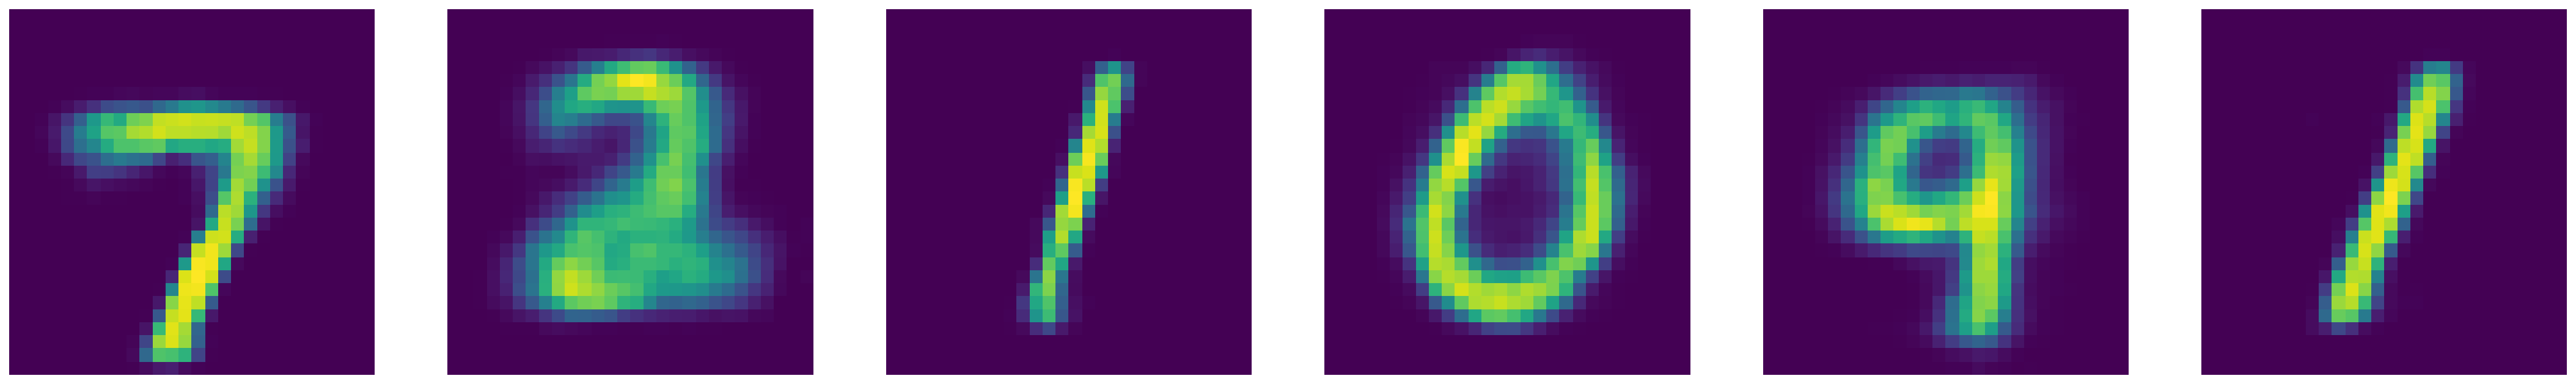
\includegraphics[width = 0.8\textwidth]{figures/cvae/mean}
		\caption{CVAE}
		\label{fig:cvae:mean}
	\end{subfigure}
	\begin{subfigure}[t]{0.5\textwidth}
		\centering
		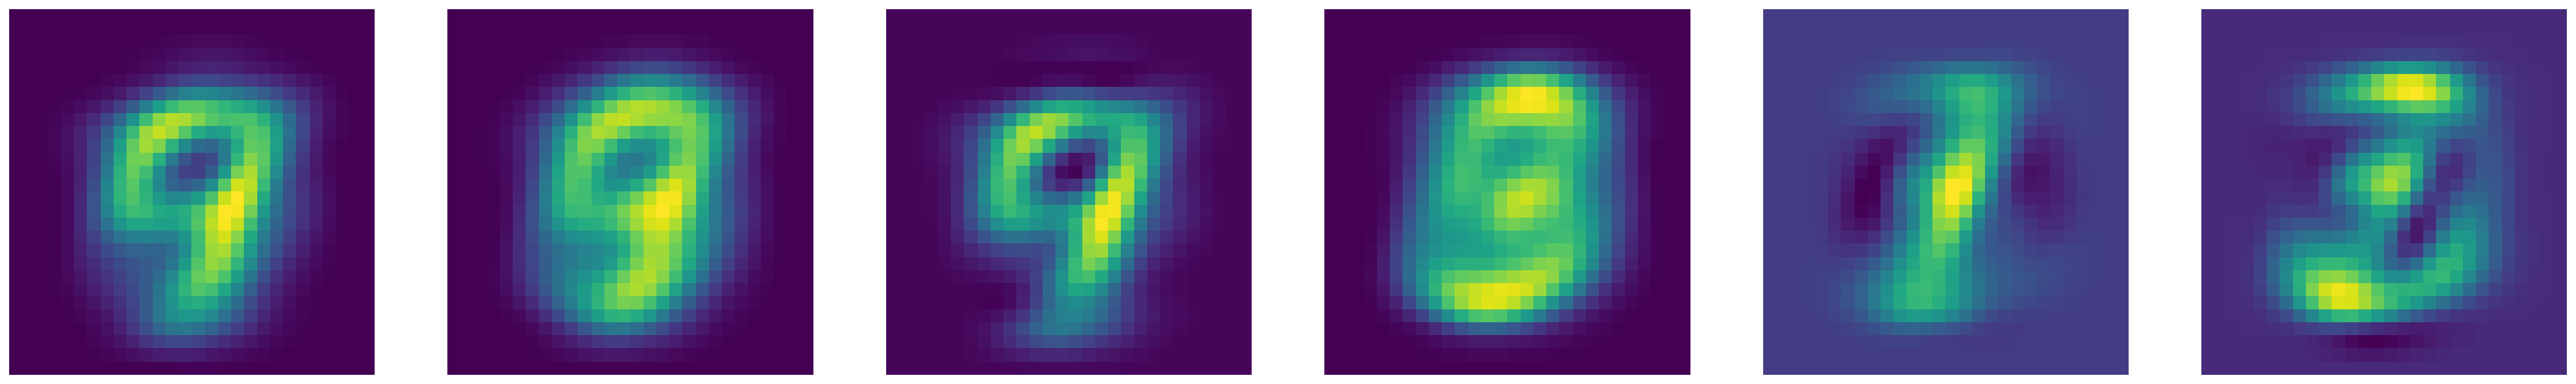
\includegraphics[width = 0.8\textwidth]{figures/ppca/mean}
		\caption{PPCA}
		\label{fig:ppca:mean}
	\end{subfigure}
	\begin{subfigure}[t]{0.5\textwidth}
		\centering
		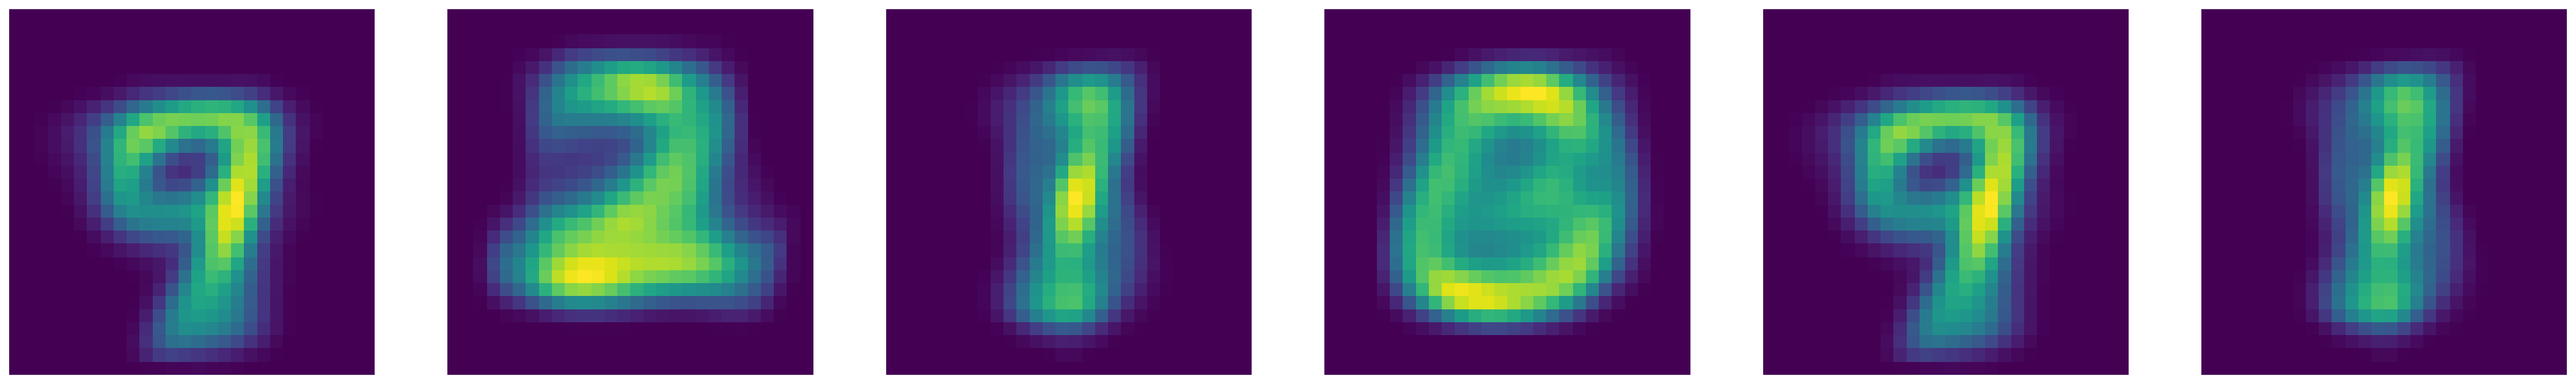
\includegraphics[width = 0.8\textwidth]{figures/gmm/mean}
		\caption{GMM}
		\label{fig:gmm:mean}
	\end{subfigure}
	
	}{%
	\caption{Comparison of MNIST test set images and corresponding mean parameters generated by density models.}
	}

	\capbtabbox{%
		\begin{tabular}{ccc}
		\toprule
		{} &  \textbf{Log-Likelihood/ELBO} &  \textbf{MSE} \\
		\midrule
		\textbf{VAE } &                 \num[round-mode=places,round-precision=4]{-1.428134e+02} &      \num[round-mode=places,round-precision=4]{0.037524} \\
		\textbf{CVAE} &                 \num[round-mode=places,round-precision=4]{-1.570527e+02} &      \num[round-mode=places,round-precision=4]{0.044375} \\
		\textbf{PPCA} &                 \num[round-mode=places,round-precision=4]{-4.329656e+03} &      \num[round-mode=places,round-precision=4]{0.055813} \\
		\textbf{GMM } &                 \num[round-mode=places,round-precision=4]{-1.066433e+07} &      \num[round-mode=places,round-precision=4]{0.058932} \\
		\bottomrule
		\end{tabular}
		
}{%
	\caption{Model performance metrics}
	\label{table:metrics}
}
	
	
\end{floatrow}
\end{figure}

\begin{figure}%[h]
	\begin{floatrow}
	\captionsetup{width=.49\linewidth}
	\ffigbox{%
	\begin{subfigure}[t]{0.45\textwidth}
		\begin{subfigure}[t]{0.49\textwidth}
			\centering
			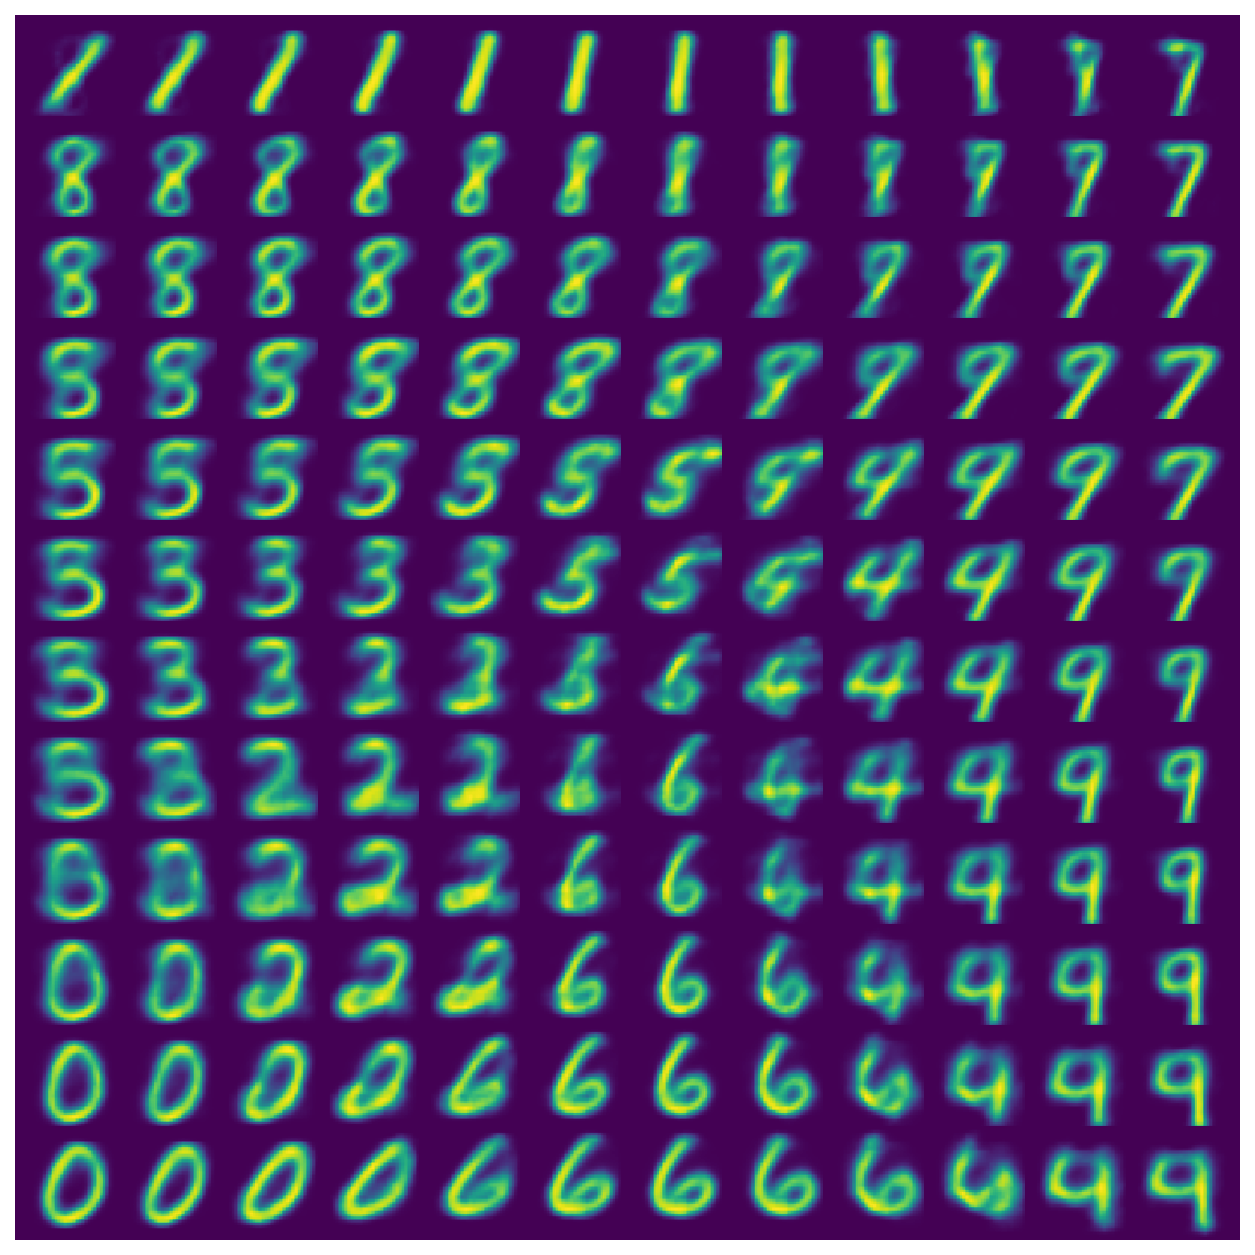
\includegraphics[width = 1\textwidth]{figures/vae/interpolation}
			\caption{VAE}
			\label{fig:vae:interpolation}
		\end{subfigure}
		\begin{subfigure}[t]{0.49\textwidth}
			\centering
			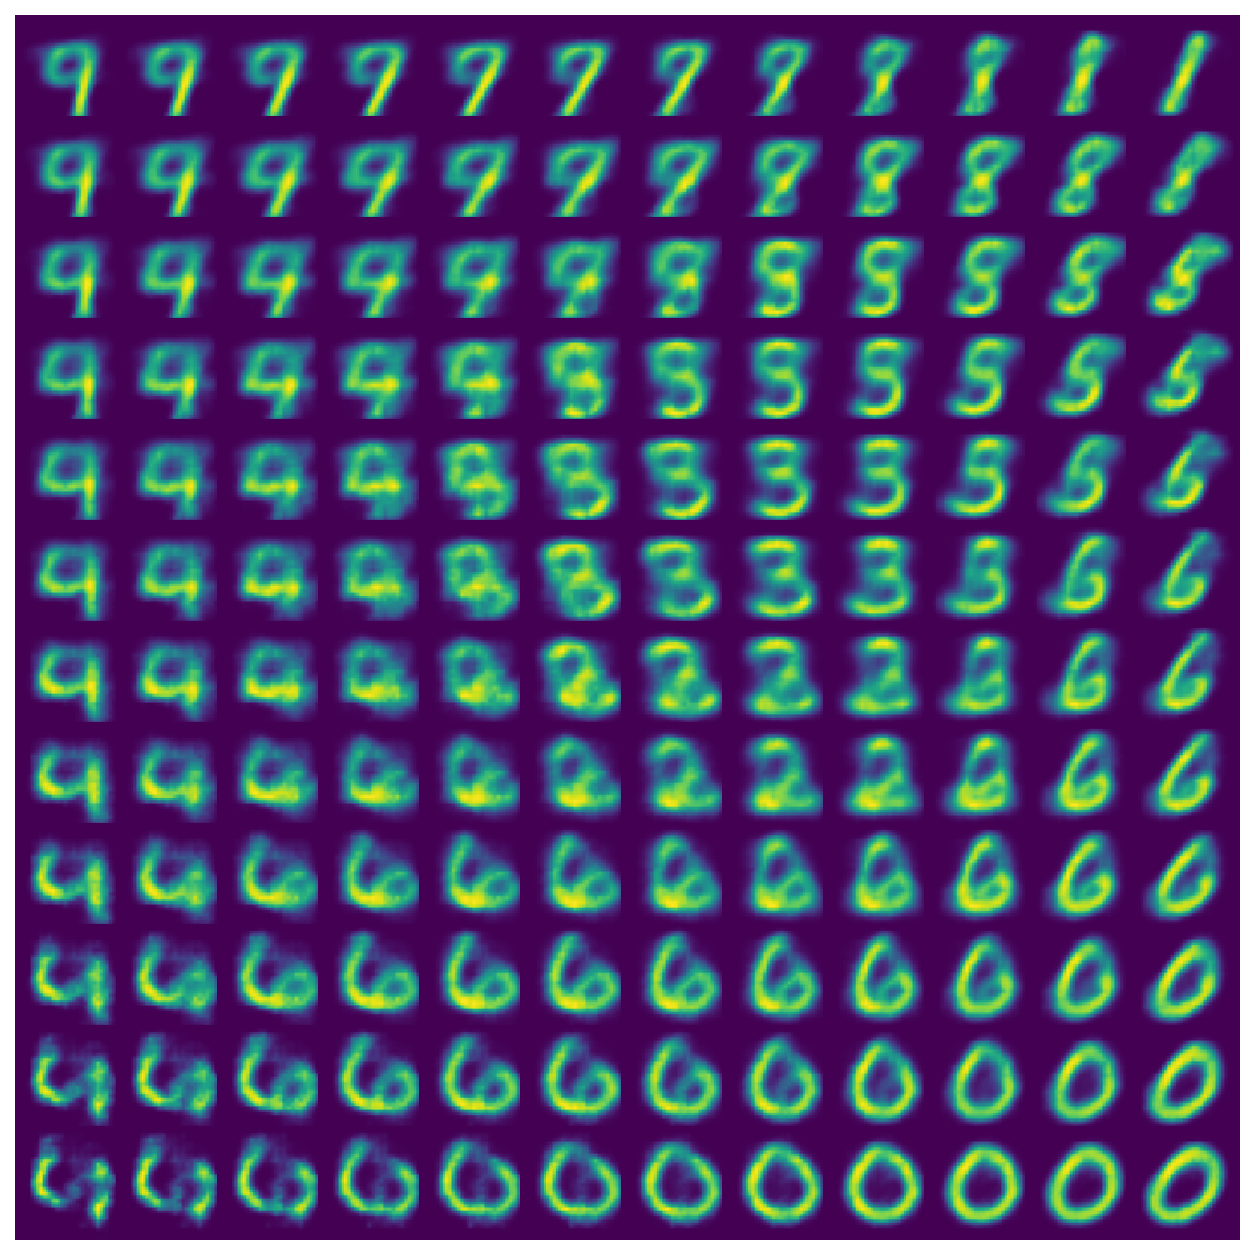
\includegraphics[width = 1\textwidth]{figures/cvae/interpolation}
			\caption{CVAE}
			\label{fig:cvae:interpolation}
		\end{subfigure}
		\begin{subfigure}[t]{0.49\textwidth}
			\centering
			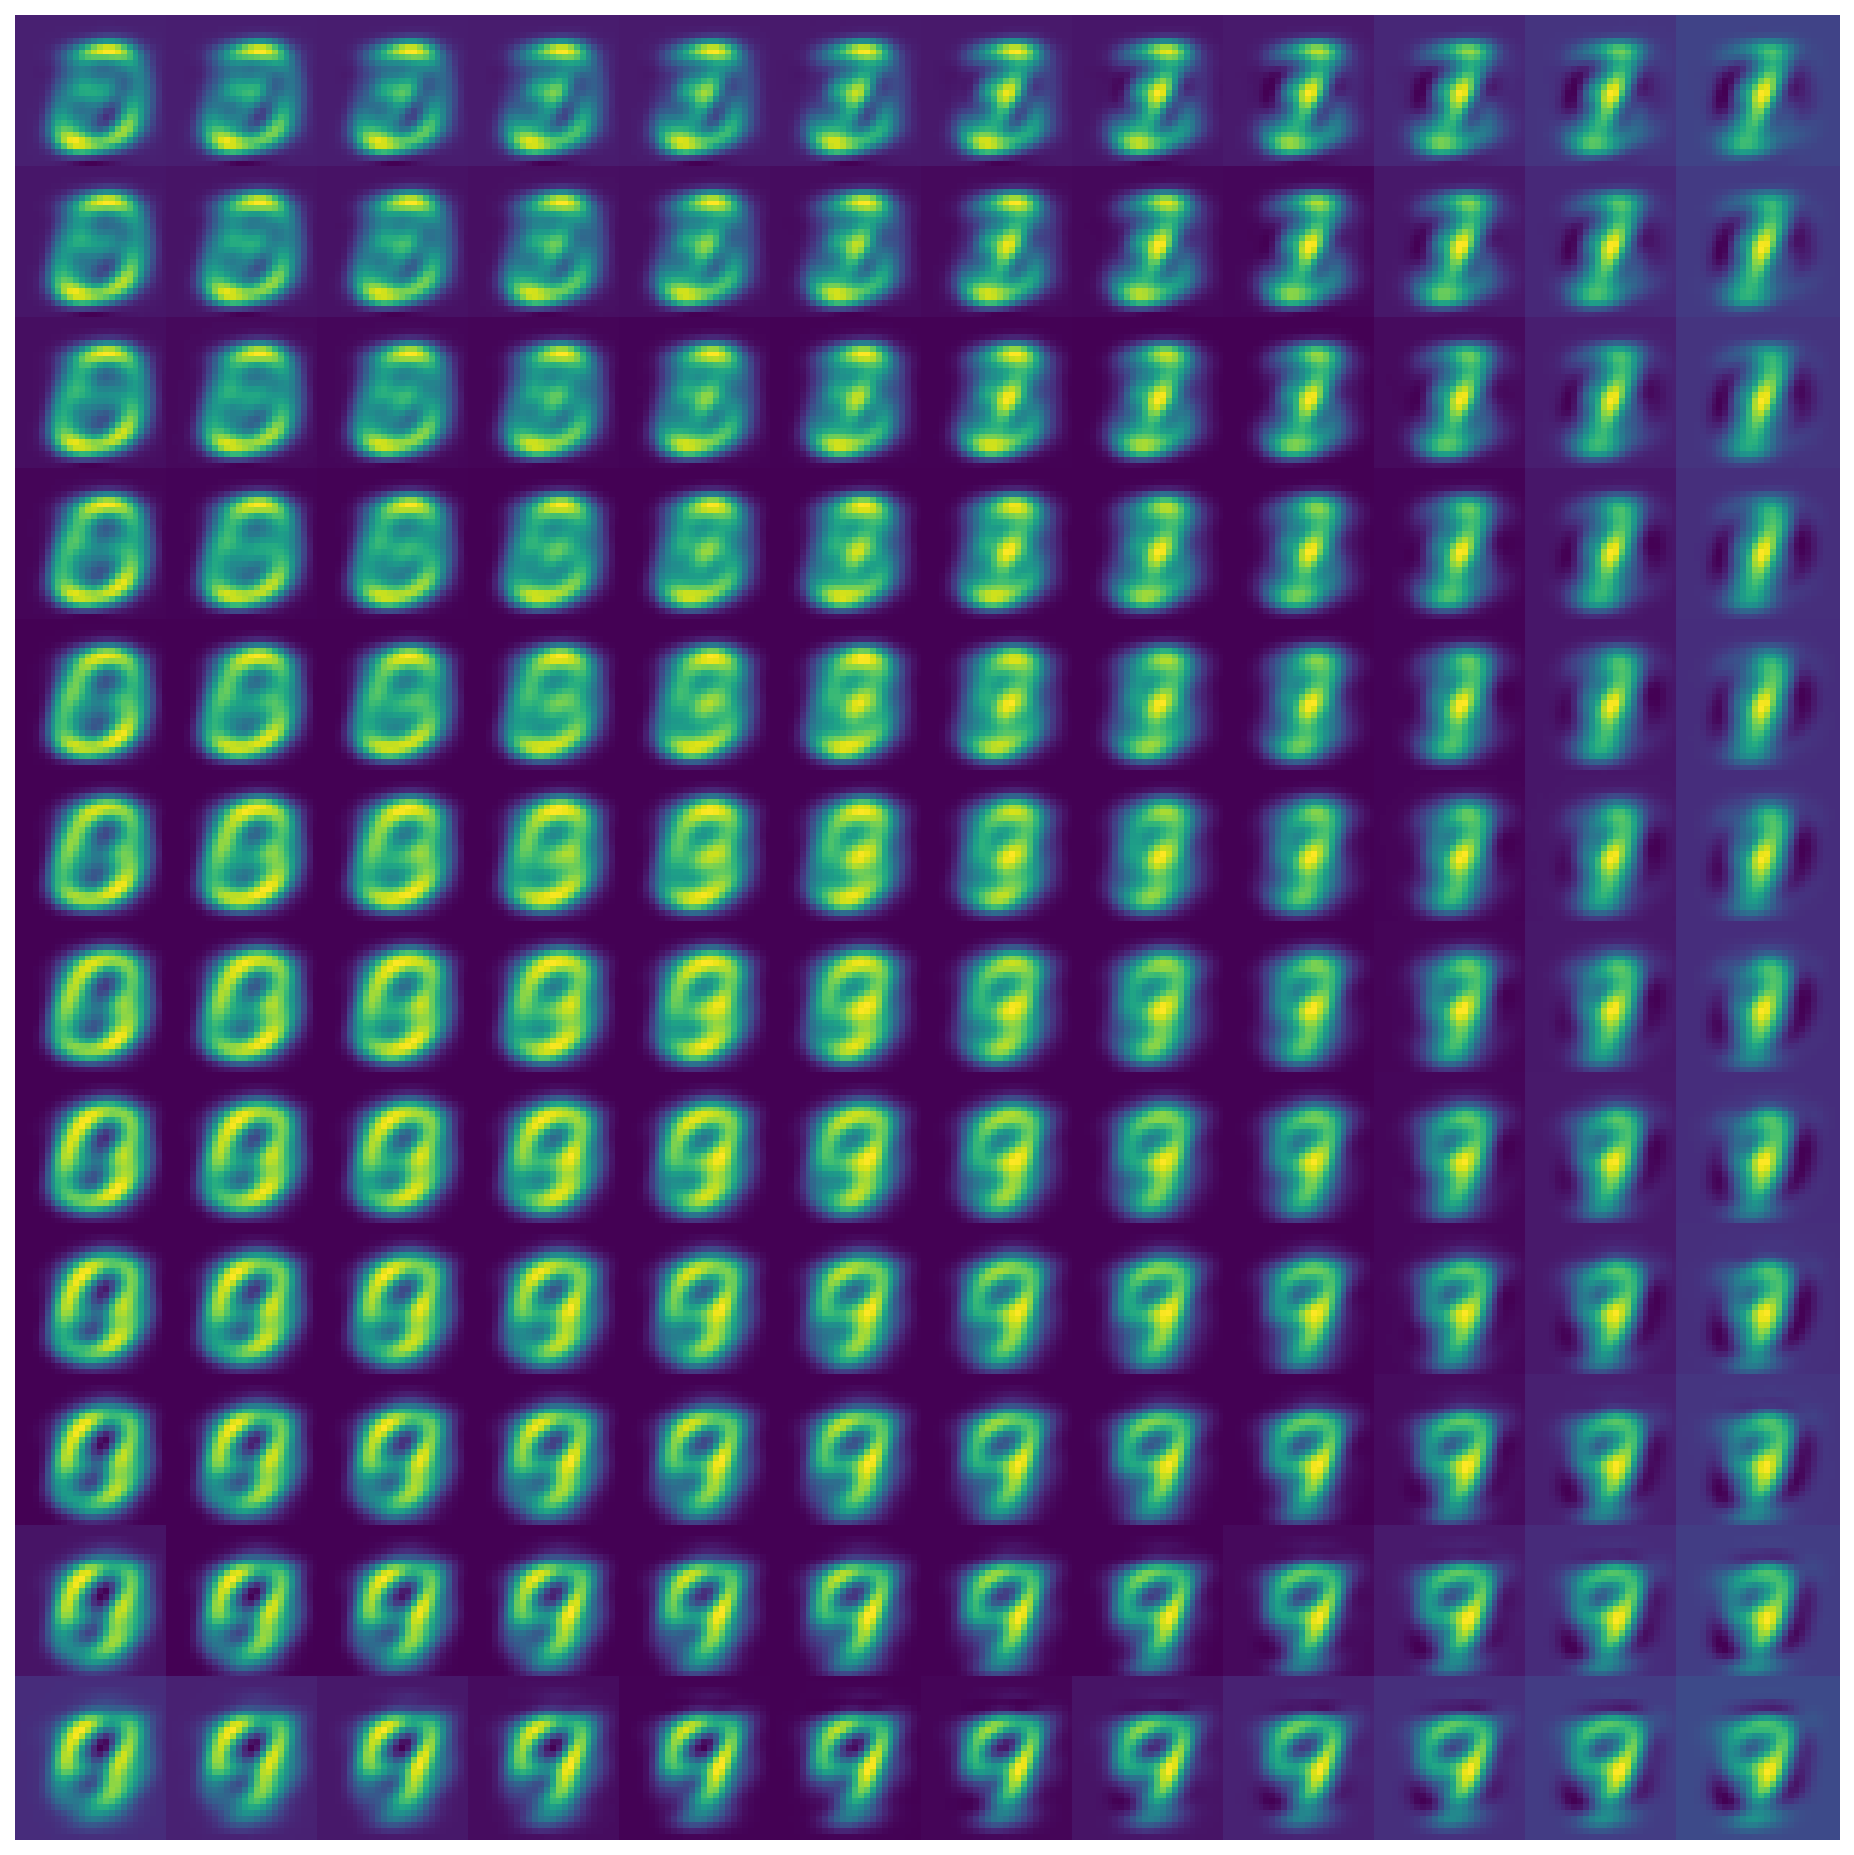
\includegraphics[width = 1\textwidth]{figures/ppca/interpolation}
			\caption{PPCA}
			\label{fig:ppca:interpolation}
		\end{subfigure}
		\begin{subfigure}[t]{0.49\textwidth}
			\centering
			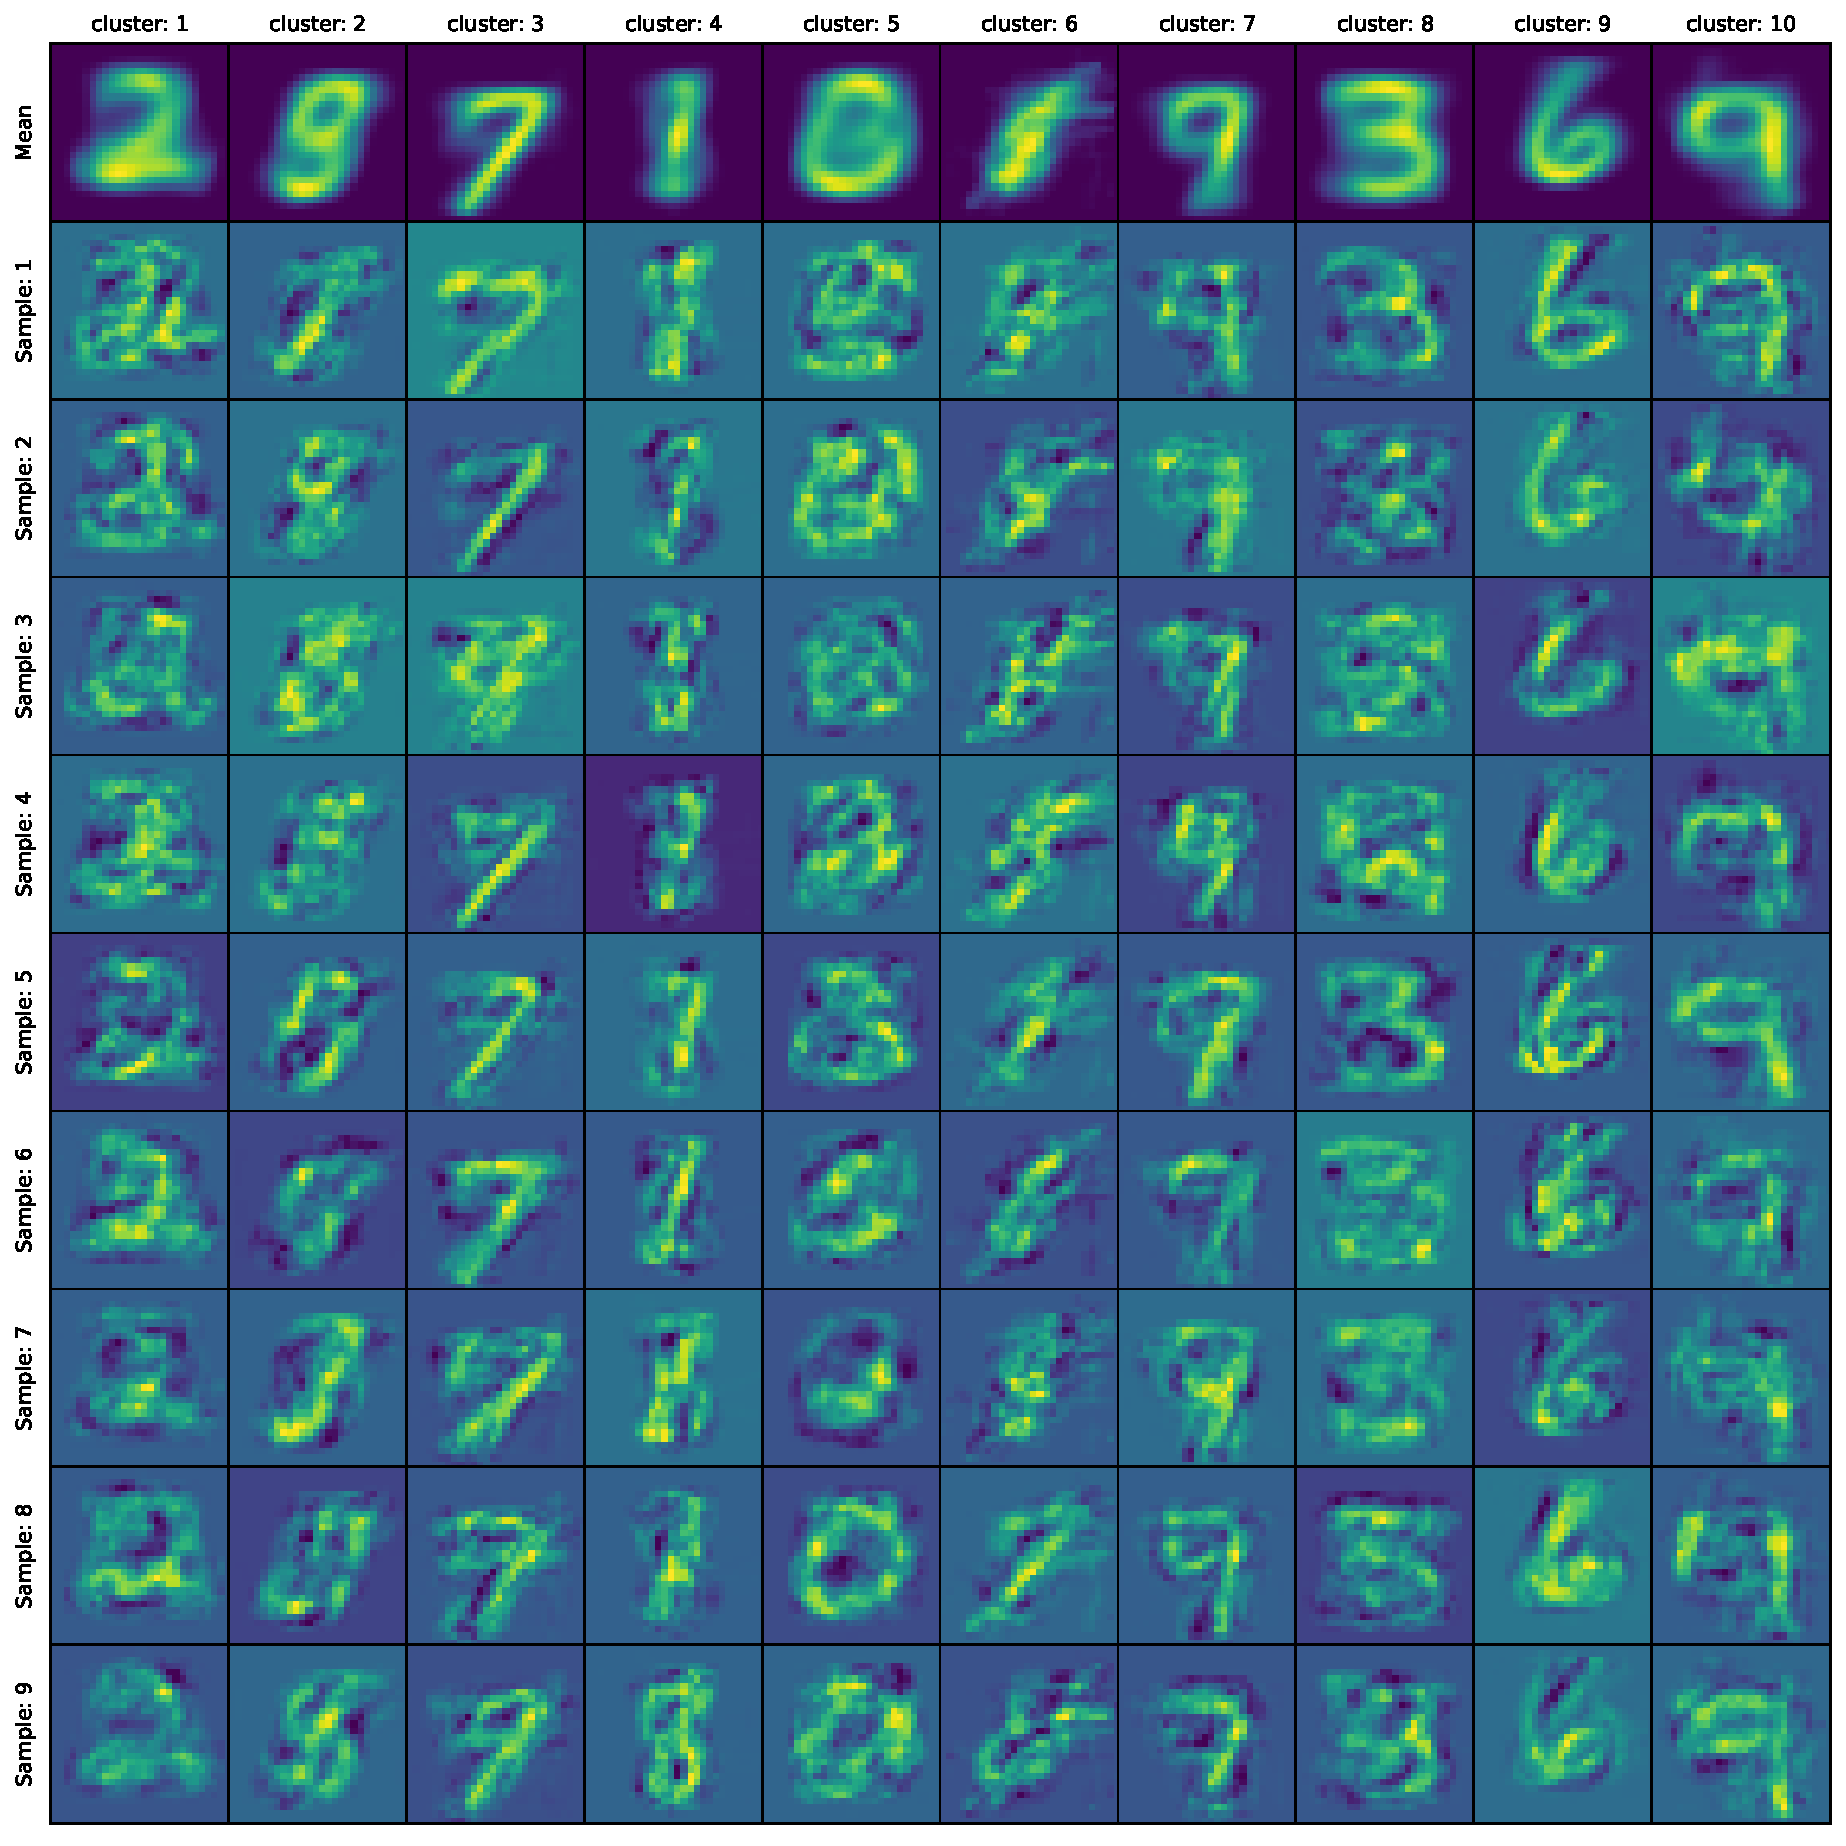
\includegraphics[width = 1\textwidth]{figures/gmm/interpolation}
			\caption{GMM}
			\label{fig:gmm:interpolation}
		\end{subfigure}	
	\end{subfigure}
	}{%
	\caption{Interpolating images from latent space variables using trained density models.}
	}
	\ffigbox{%
\begin{subfigure}[t]{0.45\textwidth}
		\begin{subfigure}[t]{0.49\textwidth}
			\centering
			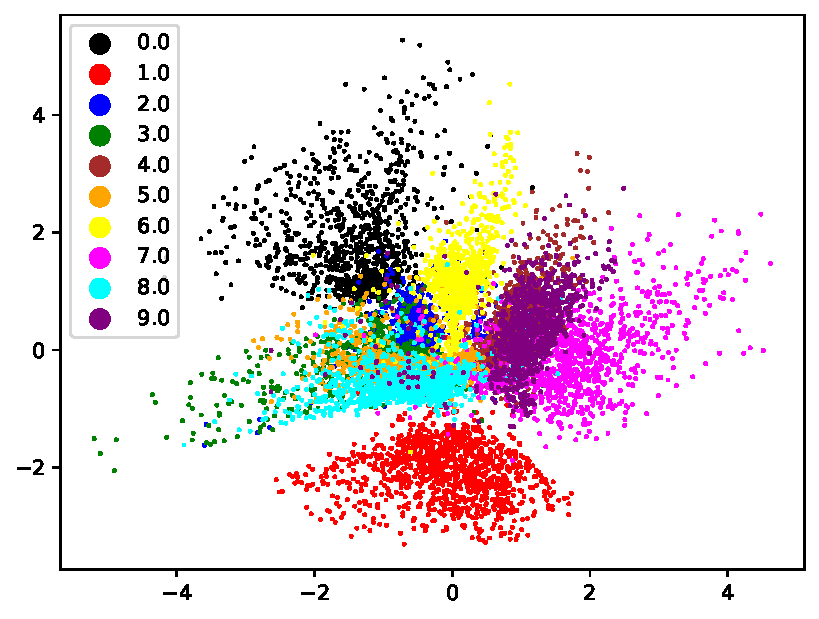
\includegraphics[width = 1\textwidth]{figures/vae/clustering}
			\caption{VAE}
			\label{fig:vae:clustering}
		\end{subfigure}
		\begin{subfigure}[t]{0.49\textwidth}
			\centering
			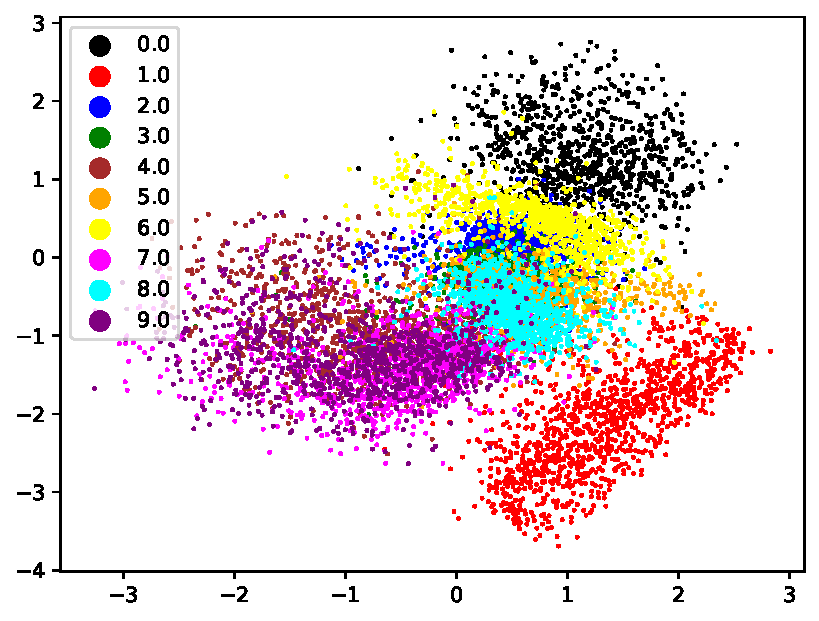
\includegraphics[width = 1\textwidth]{figures/cvae/clustering}
			\caption{CVAE}
			\label{fig:cvae:clustering}
		\end{subfigure}
		\begin{subfigure}[t]{0.49\textwidth}
			\centering
			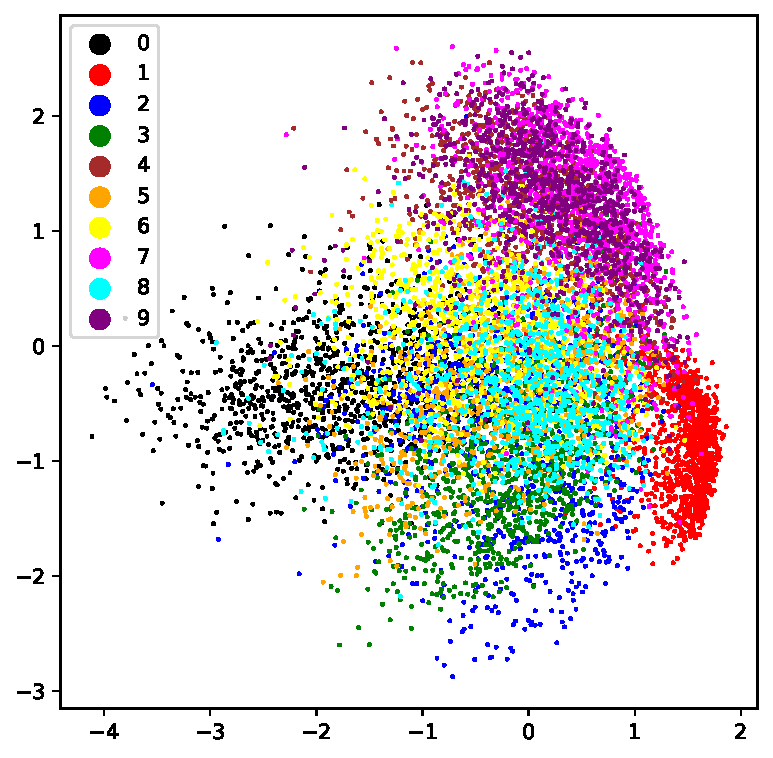
\includegraphics[width = 1\textwidth]{figures/ppca/clustering}
			\caption{PPCA}
			\label{fig:ppca:clustering}
		\end{subfigure}
		\begin{subfigure}[t]{0.49\textwidth}
			\centering
			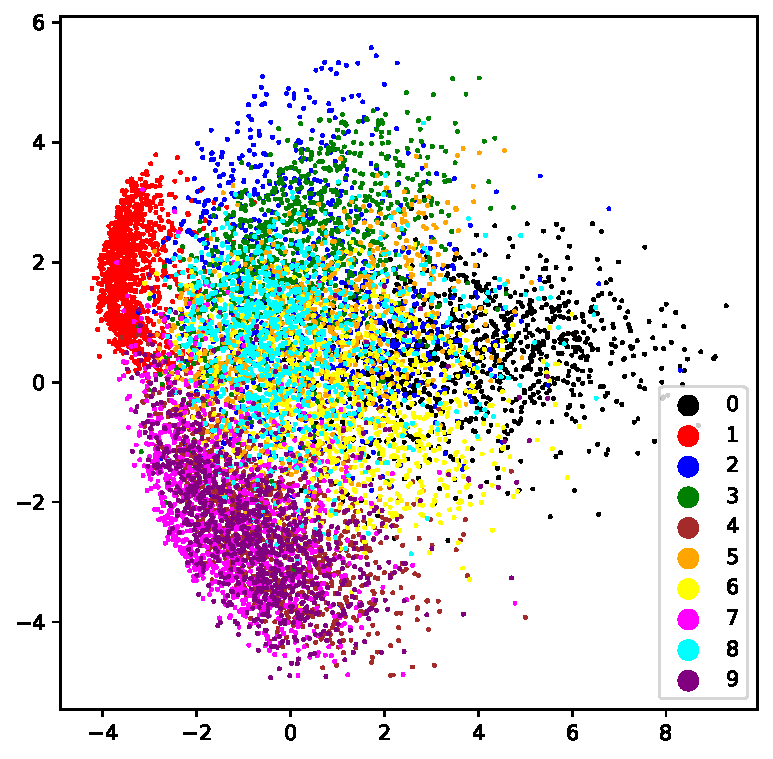
\includegraphics[width = 1\textwidth]{figures/gmm/clustering}
			\caption{GMM}
			\label{fig:gmm:clustering}
		\end{subfigure}
	\end{subfigure}
	}{%
	\caption{Clustering on MNIST test data (projection to latent space) using trained density models.}
	}
\end{floatrow}
\end{figure}

%\begin{table}
\centering
\caption{Model performance metrics}
\label{table:metrics}
\begin{tabular}{ccc}
\toprule
{} &  \textbf{Log-Likelihood/ELBO} &  \textbf{MSE} \\
\midrule
\textbf{VAE } &                   -145.122048 &      0.000305 \\
\textbf{CVAE} &                   -157.241749 &      0.000352 \\
\textbf{PPCA} &                  -4329.655559 &   3620.035365 \\
\bottomrule
\end{tabular}
\end{table}

\section{Function fitting}
\subsection{Fitting a GP with Pyro}
We have implemented a full Bayesian GP modeling approach with
Pyro. We have applied our implementation to the dataset $\mathcal{D}$ described in the assignment text.
We use NUTS, with a Gaussian RBF kernel, to sample from the posterior $p(\theta | \mathcal{D})$. The priors used for the kernel parameters $\sigma^2_l$ and $\sigma^2_s$ are the ones given in the assignment text.
For hyperparameters, we use $W = 100$ warmup steps and $C = 4$ chains.
In \cref{fig:gp:analysis} we show the ESS and r\_hat values computed for our trained model. We achieve ESS values of above 400, which indicates that our model approximates the posterior distributions of the actual parameters well. Furthermore, we have r\_hat values of 1.01 for both parameters, indicating that the sampling has converged.
\begin{figure}[H]
\begin{tabular}{l l l}
$\sigma^2_l$ & & \\ \midrule
& ESS bulk & 412.0 \\
& ESS tail & 725.0 \\
& r\_hat & 1.01\\ 
$\sigma^2_p$ & & \\\midrule
& ESS bulk & 534.0 \\
& ESS tail & 614.0 \\
& r\_hat & 1.01\\
\end{tabular}
\caption{Effective sample size (ESS) and r\_hat values calculated with Arviz}
\end{figure}
\begin{figure}[H]
    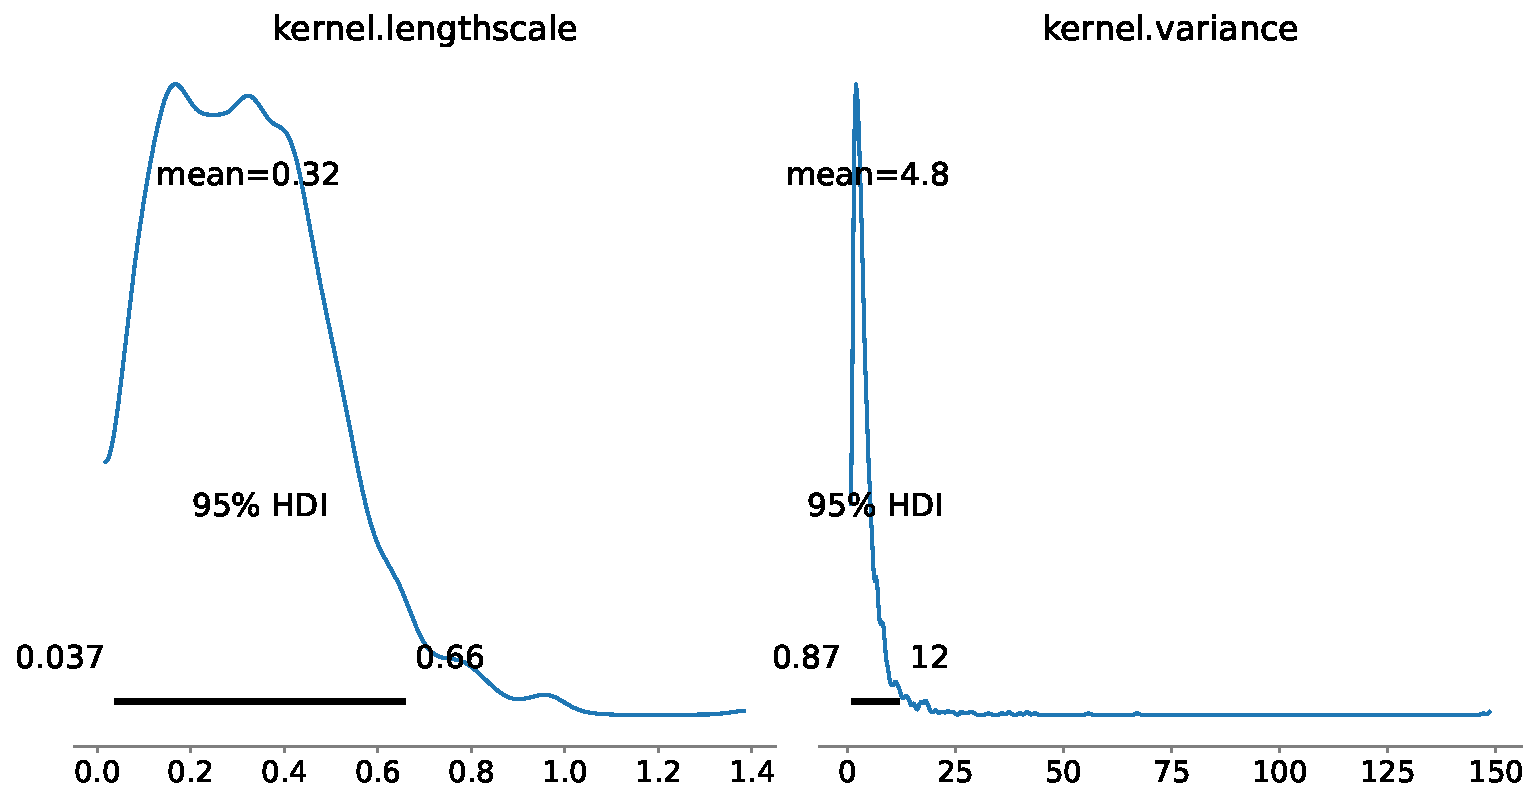
\includegraphics[width=0.49\textwidth]{figures/gp/sample_analysis.pdf}
    \caption{Plot showing the posterior densities of the RBF kernel's learned parameters}
    \label{fig:gp:sample_analysis}
\end{figure}
In \cref{fig:gp:loglog} we show 500 samples from $p(\theta|\mathcal{D})$ from each chain, and in \cref{fig:gp:plot1} we show $p(f^*|x^*, \mathcal{D})$ along with its confidence interval and mean.
\begin{figure}[H]
    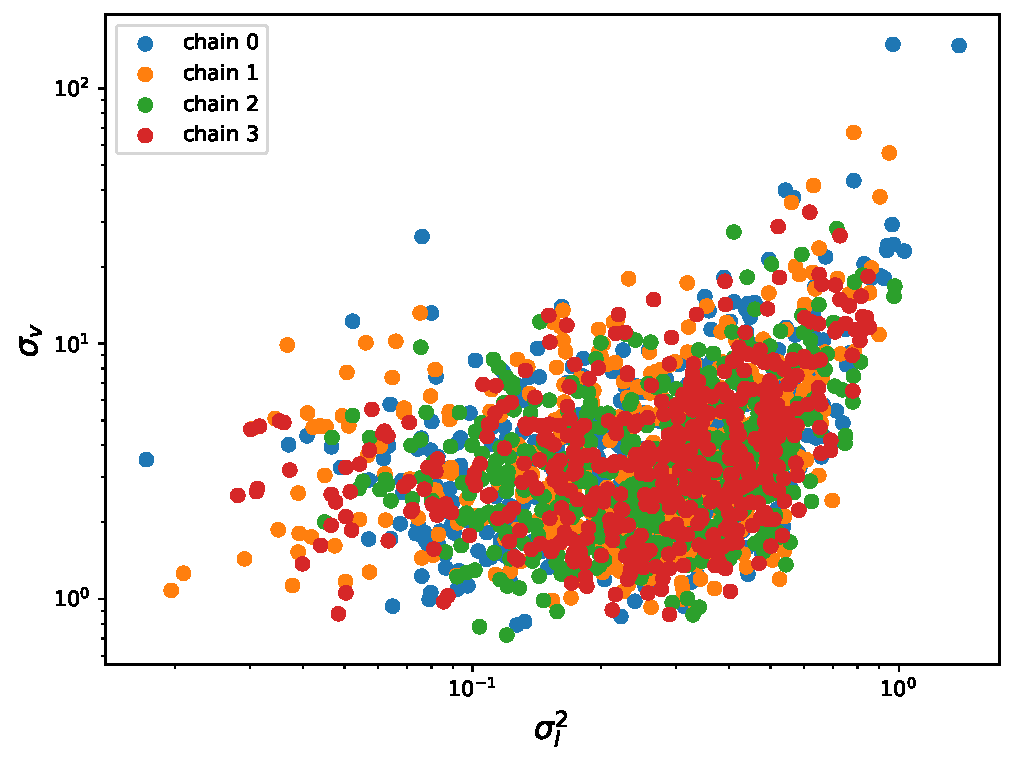
\includegraphics[width=0.49\textwidth]{figures/gp/loglogscale.pdf}
    \caption{Scatter plot on log-log-scale of $N = 500$ samples from $p(\theta | \mathcal{D})$ from 4 chains}
    \label{fig:gp:analysis}
\end{figure}
\begin{figure}[H]
    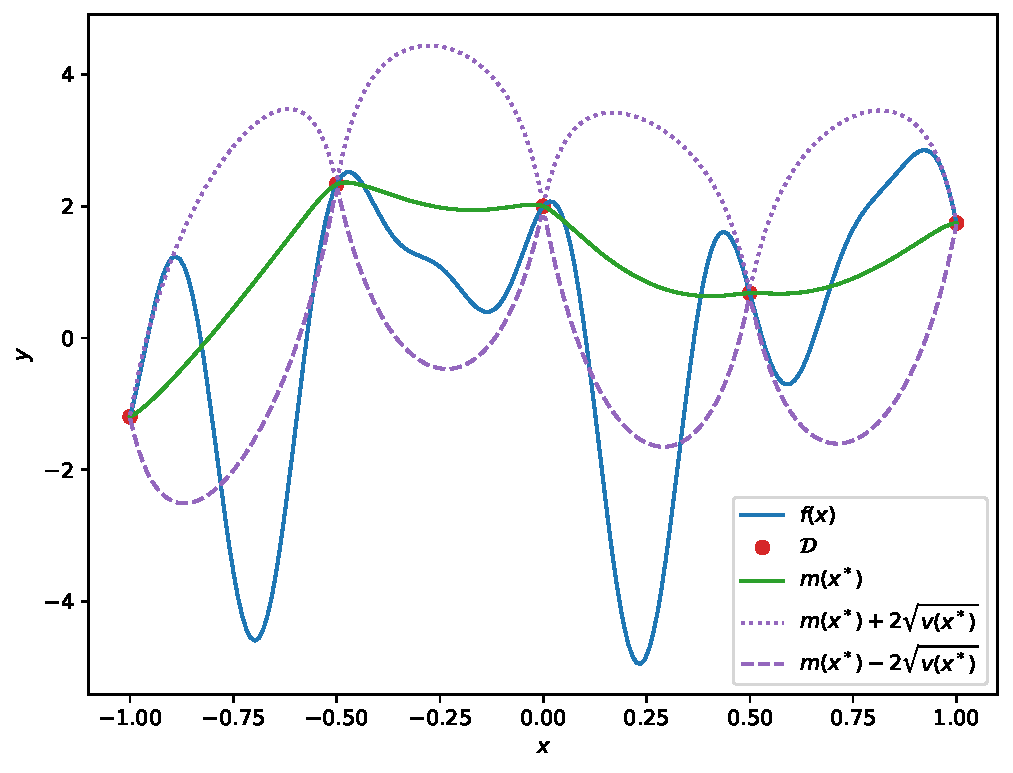
\includegraphics[width=0.49\textwidth]{figures/gp/plot.pdf}
    \caption{Plot of $p(f^*|x^*,\mathcal{D})$ along with its mean and confidence interval}
\end{figure}
\subsection{Bayesian Optimization}
In \cref{fig:gp:bayesianloop} we show the results from running our Bayesian optimization loop. We see that our implementation indeed is capable of finding the global minimum of $f$,
however, from running the optimization loop multiple times, we notice that we are not able to reliably find the global minimum of $f$. Sometimes the algorithm gets stuck in a local minimum and is never able to escape. This even happens from the first iteration in some cases. Furthermore, we also have intermittent numerical stability problems. In an attempt to address these issues, we have tried a multitude of the different kernels supplied by the Pyro library, while keeping the original prior supplied to us. However, changing the kernel made no difference, and in some cases led to worse results than we observed with the RBF kernel.

\begin{figure}%[H]
    \begin{subfigure}[t]{0.32\textwidth}
        \centering
        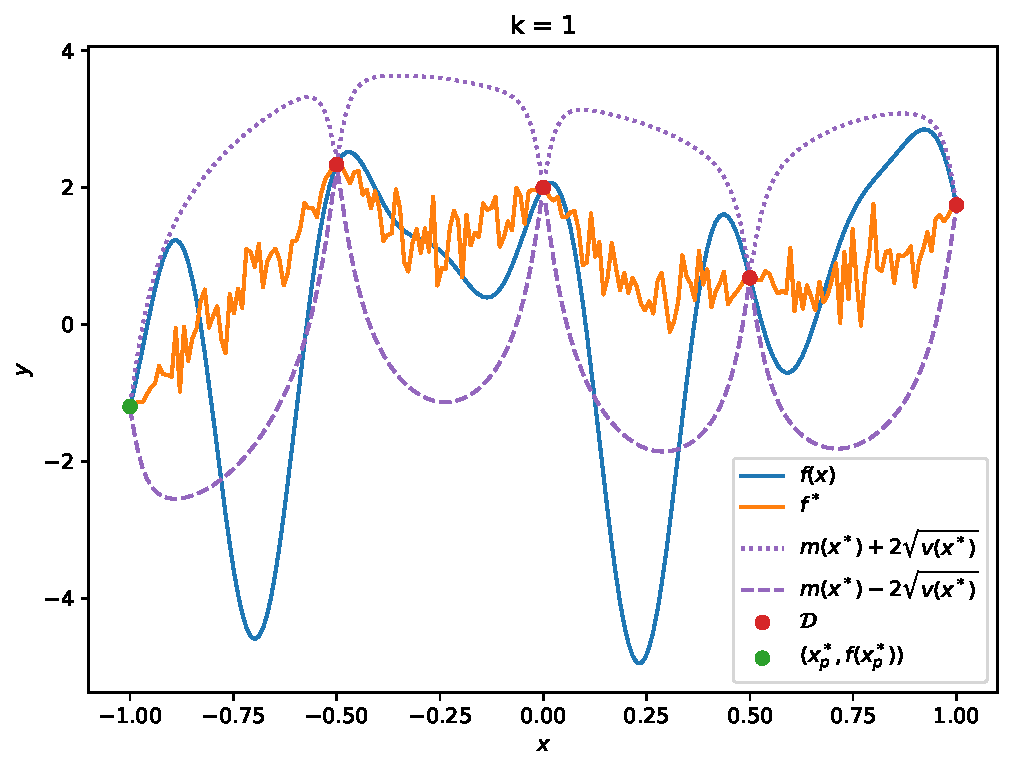
\includegraphics[width=\textwidth]{figures/gp/b2-k_1.pdf}
    \end{subfigure}
    \begin{subfigure}[t]{0.32\textwidth}
        \centering
        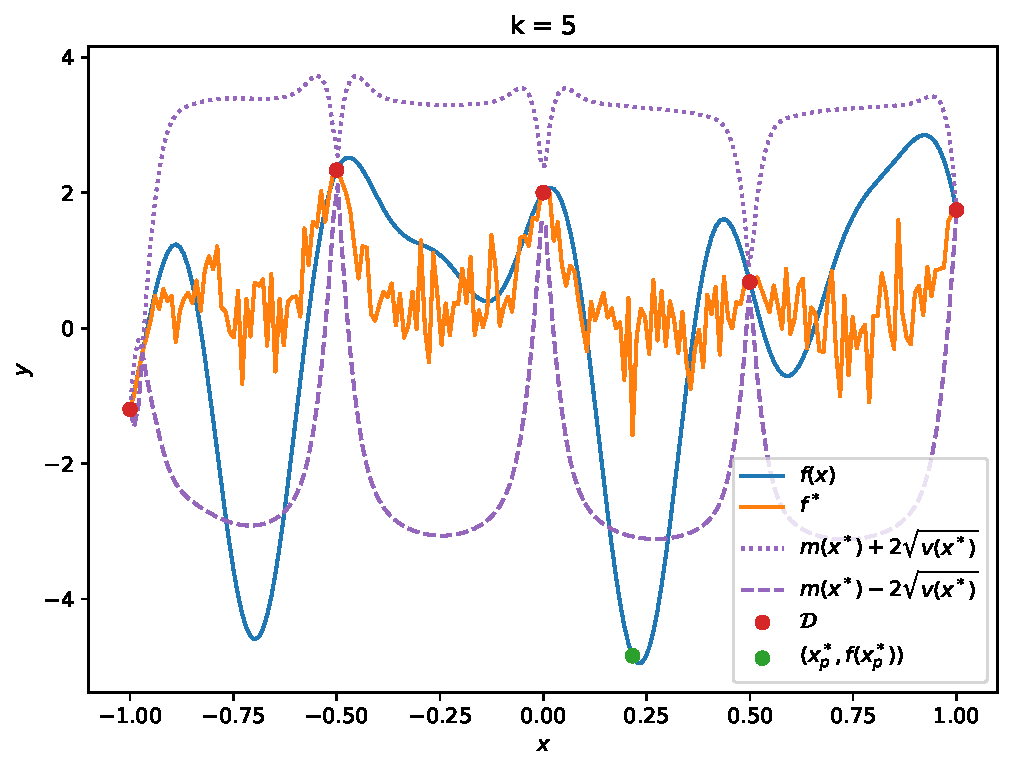
\includegraphics[width=\textwidth]{figures/gp/b2-k_5.pdf}
    \end{subfigure}
    \begin{subfigure}[t]{0.32\textwidth}
        \centering
        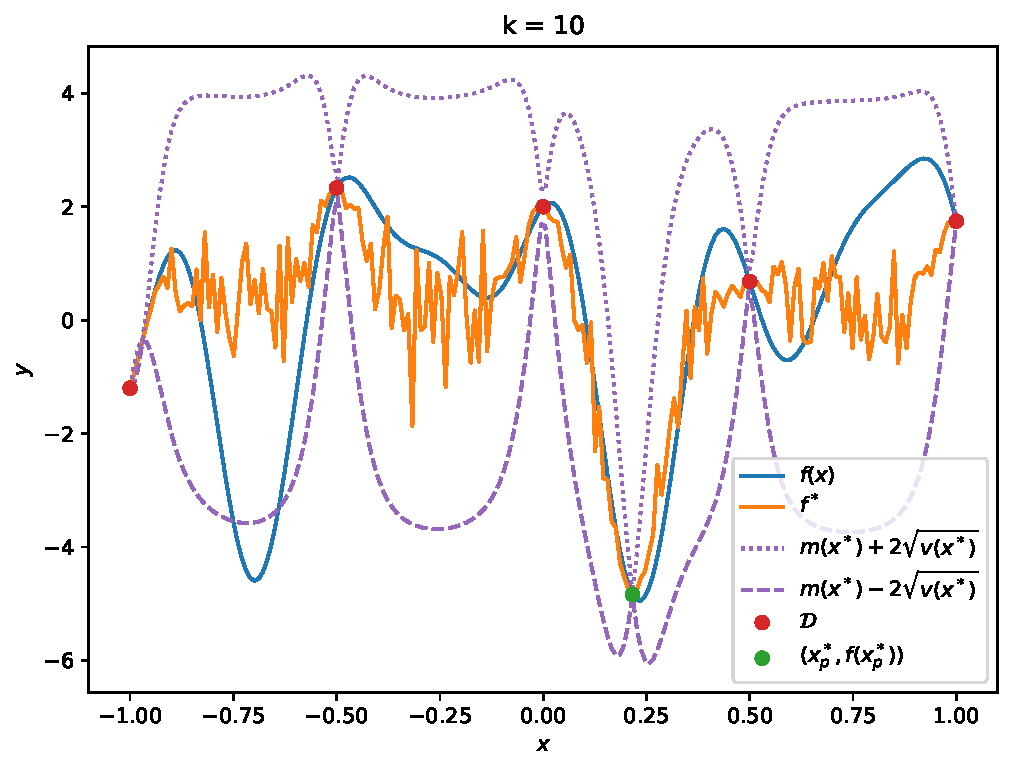
\includegraphics[width=\textwidth]{figures/gp/b2-k_10.pdf}
    \end{subfigure}
    \caption{Plots from running our Bayesian optimization loop at iteration $k$}
    \label{fig:gp:bayesianloop}
\end{figure}
\input{sections/B.tex}
\bibliographystyle{unsrtnat}
\bibliography{references.bib}

\end{document}